\documentclass[11pt, titlepage]{article}
\usepackage{amsmath,amsthm,amssymb}
\usepackage{hyperref, pgf, tikz}
\usepackage{fancyhdr}
\usetikzlibrary{arrows}
\usepackage[margin=1.25in]{geometry}
\usepackage{graphicx}                     
\pagestyle{fancy}
\usepackage{array}
%\usepackage{wrapfig}

\lhead{Lab \#03}
\rhead{\thepage}
\cfoot{}

\title{\Huge{The Addition and Resolution of Vectors: The Force Table} \\ \ \\ \huge Lab \#03}
\author{\Large{Alon Levin} \\ \emph{Lab Partners: Sophia Zheng, Avery Karlin}}
\date{\today}
\begin{document}

\maketitle

\begin{center}
\LARGE The Addtion and Resolution of Vectors: The Force Table
\end{center}

\section*{Objective}
The objectives of this lab are to learn two methods of adding sets of vectors (graphically and analytically) and thus to foster an appreciation of the differences between the two approaches.

\section*{Introduction}
A \textbf{vector} is a mathemaitcal concept which represents a quantity that has both a magnitude and a direction, unlike a \textbf{scalar} which has only a magnitude. Therefore, the process of adding vectors is more complex as well; there are two ways to find a vector sum: using the graphical method, or using the analytical method. 

\subsection*{Graphical Method}
Vectors are represented graphically as arrows, with the length proportional to the magnitude and the direction represented by the direction the arrowhead points in. As can be seen in Fig. \ref{fig:1}, the graphical method can be approached in three ways.
\begin{figure}[!ht]
\centering
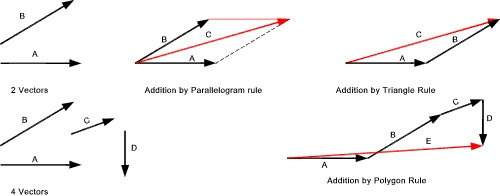
\includegraphics[scale=1, angle=0]{lab03_graphicvectors.jpg}
\caption{Three methods for graphical vector addition \label{fig:1}}
\end{figure} 
\begin{description}
	\item[Parallelogram] Given two vectors $\mathbf{A ~\text{and} ~B}$, a parallelogram could be constructed with $\mathbf{A} ~\text{and} ~\mathbf{B}$ as adjacent sides. The arrow diagonal of the parallelogram $\mathbf{R}$ is the resultant of $\mathbf{A} + \mathbf{B}$. In Fig. \ref{fig:1}, $\mathbf{R} ~\text{is denoted as} ~\mathbf{C}$.
	\item[Triangle] Given two vectors $\mathbf{A ~\text{and} ~B}$, the ``tail'' of $\mathbf{B}$ could be attached from the ``head'' of $\mathbf{A}$. The vector drawn from the tail of $\mathbf{A} ~\text{to the head of} ~\mathbf{B}$ is the resultant $\mathbf{R}$ of $\mathbf{A} + \mathbf{B}$. In Fig. \ref{fig:1}, $\mathbf{R} ~\text{is denoted as} ~\mathbf{C}$.
	\item[Polygon] For situations in which more than two vectors are added, the ``head-to-tail'' method employed in the \textbf{Triangle rule} can be employed repeatedly to form a polygon constructed of vectors. In Fig. \ref{fig:1}, $\mathbf{R} ~\text{is denoted as} ~\mathbf{E}$.
\end{description}

\section*{Procedure}

\pagebreak
\begin{figure}[!ht]
\centering
%\vspace*{1.5cm}
%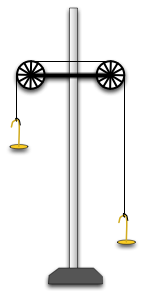
\includegraphics[scale=1.5, angle=0]{lab1.jpg}
\caption{Setup used for this experiment}
\end{figure}

\pagebreak
\section*{Data}
\begin{center}
%\begin{tabular}

%\end{tabular}
\begin{figure}[!ht]
\caption{caption}
\end{figure}
\end{center}

\pagebreak
\section*{Discussion}
\subsection*{Sample Calculations}

\subsection*{Analysis}

\section*{Conclusion}

\end{document}